\nonstopmode
\documentclass[a4paper,UKenglish,cleveref, autoref]{lipics-v2019}

\usepackage{amsmath,amssymb,amsthm,mathtools}
\usepackage[linesnumbered, ruled]{algorithm2e}
\usepackage[final]{microtype}
\usepackage[final]{hyperref}
\usepackage[inline]{enumitem}
\usepackage{subcaption}

% ERR FIX
\usepackage[T1]{fontenc}  


% DEBUG
\usepackage{lipsum}
\usepackage{fullpage}
\usepackage{lineno}
\linenumbers

% EXTRA
\usepackage{authblk}

\tikzset{every picture/.style={
	very thick
% 	,>=Latex
	,>=stealth
}}

% LINES
\tikzset{
	line blue/.style={blue,dotted}
	,line red/.style={red,dashed}
	,line brown/.style={brown,dashdotted}
	,line teal/.style={teal,dashdotdotted}
}

% NODE
\tikzset{default node/.style={
	draw, 
	circle,
	inner sep=0mm,
	minimum size=5mm,
	very thick,
	font=\small
}}

\tikzset{
colored node/.style={line width=1.6pt, star, minimum size=9mm,inner sep=0pt,scale=0.9,}, 
red node/.style={colored node, draw=red, star points=2},
blue node/.style={colored node, draw=blue, star points=3},
green node/.style={colored node, draw=green, star points=4},
black node/.style={colored node, draw=black, star points=5},
orange node/.style={colored node, draw=orange, star points=6},
brown node/.style={colored node, draw=brown, star points=8},
teal node/.style={colored node, draw=teal, star points=10},
violet node/.style={colored node, draw=violet, star points=12},
olive node/.style={colored node, draw=olive, star points=14},
cyan node/.style={colored node, draw=cyan, star points=18},
}

% EDGES
\tikzset{
	light/.style={
		thin,
		gray,
	},
	path/.style={
		light,
		decorate, 
		decoration={snake, segment length=18pt},
	},
	brace/.style={
		decorate,
		decoration={brace, amplitude=5},
		-,
	},
}

\tikzset{e1/.style={cyan}}
\tikzset{e2/.style={green, loosely dash dot dot}}
\tikzset{e3/.style={blue, loosely dotted}}
\tikzset{e4/.style={loosely dashed}}
\tikzset{e5/.style={red, loosely dashed}}
\tikzset{e6/.style={orange, loosely dash dot}}

% LABELS
\tikzset{
	label/.style={
		rectangle,
		draw=none,
		sloped,
		midway,
		fill=white,
		inner sep=2pt,
		minimum height=0,
		minimum width=0,
	},
	label above/.style={
		label,
		above,
	},
	label below/.style={
		label,
		below,
	},
	label inside/.style={
		label,
		fill=white,
		draw=black,
	},
}


% MISC
\tikzset{
	cloud/.style={
		-,
		decorate, 
		decoration={
			snake, 
			segment length=3mm,
			amplitude=.5mm,
		},
	}
	,outline/.style={
		dotted
		,purple
		,very thick	
	}
	,packing/.style={
		outline
		,-
	}
	,m/.style={blue, dashed}
}




\DeclareMathOperator*{\argmin}{arg\,min}
\DeclareMathOperator*{\argmax}{arg\,max}

\def\R{\mathbb{R}}
\def\N{\mathbb{N}}

\newtheorem{observation}{Observation}
\newtheorem{lemma}{Lemma}
\newtheorem{theorem}{Theorem}

\newcommand{\defeq}{\vcentcolon=}

\newcommand\todo[1]{\textcolor{red}{TODO }{#1}}
% \renewcommand\todo[1]{}

\title{A Fast and Simple Algorithm for Submodular Maximization with a Knapsack Constraint}
\titlerunning{A Fast and Simple Algorithm for Submodular Knapsack}

\author{Ariel Kulik}{Department of Computer Science, Technion, Haifa, Israel}{kulik@cs.technion.ac.il}{}{}
\author{Gilad Kutiel}{Department of Computer Science, Technion, Haifa, Israel}{gkutiel@cs.technion.ac.il}{}{}
\author{Roy Schwartz}{Department of Computer Science, Technion, Haifa, Israel}{schwartz@cs.technion.ac.il}{}{}
\authorrunning{A.\,Kulik and G.\,Kutiel and R.\,Schwartz}

\Copyright{Ariel Kulik and Gilad Kutiel and Roy Schwartz}
\ccsdesc{}

%\ccsdesc[100]{ {\color{red}{TBD}} }
%\ccsdesc[100]{ {\color{red}{TBD}} }

\ccsdesc[100]{Theory of computation~Submodular optimization and polymatroids}
\ccsdesc[100]{Theory of computation~Approximation algorithms analysis}

\keywords{knapsack, submodular function, approximation algorithm}

%\category{}

%\relatedversion{}

%\supplement{}

\nolinenumbers



\newcommand{\SK}{{\textsc{Submodular Knapsack}}\xspace}



\begin{document}
\maketitle

\begin{abstract}
We consider the problem of maximizing a monotone submodular function with a knapsack constraint.
In this work we aim at finding fast and simple algorithms for the problem.
Previously, the best fast and simple algorithm is that of Khuller {\em et. al.} [IPL`99] which runs in time $O(n^2)$ and achieves an approximation guarantee of $(1-e^{-\nicefrac[]{1}{2}})\approx 0.393 $.
We present a new fast and simple algorithm which retains the same running time and has an improved approximation guarantee of $0.4536$.
%At the heart of our analysis lies a method that enables us to better analyze the greedy ``bang per buck'' algorithm in the presence of elements with varying cost.
Moreover, we present a general method for ``amplifying'' the approximation factor of any algorithm for the problem, while losing little in the constants of the running time.
Applying this amplification to our new algorithm enables us to further improve the results obtained.
We believe that our amplification method might be of independent interest.

\end{abstract}

\section{Introduction}
Submodularity is a fundamental mathematical notion that captures the concept of economy of scale and is prevalent in many areas of science and technology.
Given a ground set $U$ a set function $f:2^U \to \mathbb{R}_+$ over $U$ is called \emph{submodular} if it has the \emph{diminishing returns} property:
$f(A \cup \{a\}) - f(A) \geq f(B \cup \{a\}) - f(B)$ for every $A \subseteq B \subseteq U$ and $a \in U \setminus B$.\footnote{
    An equivalent definition is: $f(A) + f(B) \geq f(A \cup B) + f(A \cup B)$ for every $A,B \in U$.
}
Submodular functions naturally arise in different disciplines such as combinatorics, graph theory, probability, game theory, and economics.
Some well known examples include coverage functions, cuts in graphs and hypergraphs, matroid rank functions, entropy, and budget additive functions.
Additionally, submodular functions play a major role in many real world applications, {\em e.g.}, the spread of influence in networks \cite{KKT03,KKT05,KKT15,MR10}, recommender systems \cite{EG11,EVSG09}, document summarization \cite{DKR13,LB10,LB11}, and information gathering \cite{GKS05,KG11,KGGK06,KGGK11,KSG08}, are just a few such examples.

Combinatorial optimization problems with a submodular objective have been the focus of intense research in the last decade as such problems provide a unifying framework that captures many fundamental problems in the theory of algorithms and numerous real world practical applications.
Examples of the former include, {\em e.g.}, Max-CUT and Max-DiCUT \cite{FG95,GW95,HZ01,H01,K72,KKMO07,LLZ02,TSSW00}, Max-$k$-Coverage \cite{F98,SW11,V01}, Max-Bisection \cite{ABG13,FJ97,HZ02,Y01}, Generalized-Assignment \cite{CK05,CKR06,FGMS06,FV06}, and Max-Facility-Location \cite{AS99,CFN77a,CFN77b}\footnote{Many of the above mentioned problems can also be found in introductory books to approximation algorithms \cite{SW11,V01}.}, whereas examples of the latter include, {\em e.g.}, pollution detection \cite{KLGVF08}, gang violence reduction \cite{SSPB14}, outbreak detection in networks \cite{LKGFFVG07}, exemplar based clustering \cite{GK10}, image segmentation \cite{KXFK11}, and recommendation diversification \cite{YG11}.

A main driving force behind the above research is the need for algorithms that not only provide provable approximation guarantees, but are also fast and  simple to implement in practice.
This need stems from the sheer scale of the applicability of submodular maximization problems in diverse disciplines, and is further amplified by the fact that many of the practical applications arise in areas such as machine learning and data mining where massive data sets and inputs are ubiquitous.\footnote{Refer to the recent book \cite{B13} and survey \cite{KG14} for additional examples and applications of submodularity in machine learning.}


%Submodularity is prevalent in many ares of science and technology, {\em e.g.}, machine learning and data mining~\cite{bach2013learning,bordeaux2014tractability}, algorithmic game theory and social networks~\cite{dughmi2009revenue,hartline2008optimal,he2015stability,kempe2003maximizing,schulz2013approximating}, and economics~\cite{ahmed2011maximizing}.
%It serves as a unifying framework capturing both classic problems in the theory of algorithms and practical applications.
%Examples of the former include, {\em e.g.}, maximum cut and maximum directed cut~\cite{goemans1995improved,Halperin:2001:CAA:365411.365412,Hastad:2001:OIR:502090.502098,Karp1972,Khot05optimalinapproximability}, maximum coverage~\cite{Feige:1998:TLN:285055.285059,KHULLER199939}, generalized assignment problem~\cite{Chekuri06apolynomial,Cohen06anefficient,Feige2006ApproximationAF,Fleischer:2006:TAA:1109557.1109624}, maximum bisection~\cite{DBLP:journals/talg/AustrinBG16,DBLP:journals/algorithmica/FriezeJ97}, and facility location~\cite{DBLP:journals/dam/AgeevS99,CORNUEJOLS1977163,doi:10.1287/mnsc.23.8.789}.
%Examples of the latter include, {\e, e.g.}, {\color{red}{ROY: ADD EXAMPLES FROM GRANT PROPOSAL}}.
%
%%The study of combinatorial optimization problems with a submodular objective has attracted much attention in the last decade.
%%A set function $f:2^\mathcal{N} \to \mathbb{R}_+$ over a ground set $\mathcal{N}$ is called \emph{submodular} if it has the \emph{diminishing returns} property:
%%$f(A \cup \{a\}) - f(A) \geq f(B \cup \{a\}) - f(B)$ for every $A \subseteq B \subseteq \mathcal{N}$ and $a \in \mathcal{N} \setminus B$\footnote{
%%    An equivalent definition is: $f(A) + f(B) \geq f(A \cup B) + f(A \cup B)$ for every $A,B \in \mathcal{N}$.
%%}
%%Submodular functions capture the principle of economy of scale, prevalent in bothe theory and real world applications.
%%Thus, it is no surprise that combinatorial optimization problems with a submodular objective arise in numerous disciplines, e.g., machine learning and data mining~\cite{bach2013learning,bordeaux2014tractability}, algorithmic game theory and social networks~\cite{dughmi2009revenue,hartline2008optimal,he2015stability,kempe2003maximizing,schulz2013approximating}, and economics~\cite{ahmed2011maximizing}.
%%Additionally, many classical problems in combinatorial optimization are in fact submodular in nature, e.g., maximum cut and maximum directed cut~\cite{goemans1995improved,Halperin:2001:CAA:365411.365412,Hastad:2001:OIR:502090.502098,Karp1972,Khot05optimalinapproximability}, maximum coverage~\cite{Feige:1998:TLN:285055.285059,KHULLER199939}, generalized assignment problem~\cite{Chekuri06apolynomial,Cohen06anefficient,Feige2006ApproximationAF,Fleischer:2006:TAA:1109557.1109624}, maximum bisection~\cite{DBLP:journals/talg/AustrinBG16,DBLP:journals/algorithmica/FriezeJ97}, and facility location~\cite{DBLP:journals/dam/AgeevS99,CORNUEJOLS1977163,doi:10.1287/mnsc.23.8.789}.

In this paper we consider the problems of maximizing a monotone\footnote{
    $f$ is monotone if $f(S) \leq f(T)$ for every $S \subseteq T \subseteq U$.
} submodular function given a knapsack constraint.
%{\color{red}{ROY: ADD APPLICATIONS SPECIFIC TO OUR PROBLEM HERE WITH A SHORT EXPLANATION}}.
In this problem we are given a ground set
$U$ of size $n$, a monotone submodular function $f:2^U \to \mathbb{R}_+$, a cost function $c:U \to \mathbb{R}_+$, and a budget $\beta$.
The goal is to find a subset of elements $S$ that maximizes $f(S)$ such that the total cost of the elements in $S$ does not exceed the budget, {\em i.e.}, $\sum _{x\in S}c(x)\leq \beta$.
For abbreviation we denote this problem by \SK.
Besides being a natural problem on its own right, capturing the classic Knapsack problem, \SK admits practical applications, {\em e.g.}, entropy maximization in graphical models \cite{krause2005note}, and document summarization \cite{LB10}.
In this work we aim to find {\em fast} and {\em simple} algorithms for the \SK problem.

We assume the standard value oracle model, where the algorithm can access the objective $f$ via queries of the form: ``what is $f(S)$?'' for every $S\subseteq U$.
The running time is the total number of value oracle queries and numerical operations performed by the algorithm. In all our algorithms the former dominates the later, and thus we are satisfied with counting the number of oracle queries alone.

Building upon the work of Khuller {\em et. al.} \cite{khuller1999budgeted}, Sviridenko \cite{sviridenko2004note} presented a tight approximation of $(1-\nicefrac[]{1}{e})\approx 0.632$ for \SK.
The algorithm of \cite{sviridenko2004note} returns the best of all subsets of $U$ of size at most three, where each subset of size three is greedily extended by the standard greedy rule that maximizes the ``bang per buck''.
This results in an impractical algorithm whose running time is $O(n^5)$.
A fast algorithm whose running time is just that of the greedy algorithm, {\em i.e.}, $O(n^2)$, was given by \cite{khuller1999budgeted} and it achieves a worse approximation of $(1-e^{-\nicefrac[]{1}{2}})\approx 0.393$.\footnote{Khuller {\em et. al.} \cite{khuller1999budgeted} considered the special case where the objective is a coverage function. This was later extended by Krause and Guestrin \cite{krause2005note} and Lin and Bilmes \cite{LB10} to a general monotone submodular objective.}


Deviating from the above combinatorial approach of \cite{khuller1999budgeted,sviridenko2004note} to \SK, Badanidiyuru and Vondr\'{a}k \cite{badanidiyuru2014fast} initiated a different line of research based on both continuous and discrete techniques.
They presented an algorithm achieving an approximation of $(1-\nicefrac[]{1}{e}-\varepsilon)$ whose running time is $O(n^2(\varepsilon ^{-1}\log n)^{\text{poly}(\varepsilon^{-1})})$, for every constant $\varepsilon >0$.
%In contrast to the combinatorial approach of \cite{khuller1999budgeted,sviridenko2004note}, Badanidiyuru and Vondr\'{a}k based their algorithm on a continuous approach.
Building upon the approach of \cite{badanidiyuru2014fast}, Ene and Nguy\~{\^{e}}n \cite{Alina2017} presented an algorithm achieving the same approximation guarantee whose running time it $O(\varepsilon^{-O(\varepsilon^{-4})}n \log^2 n)$.
Both algorithms of \cite{badanidiyuru2014fast,Alina2017} are theoretically interesting and appealing, as they require the introduction of novel ideas that enable one to extrapolate between the discrete and continuous approaches.
Unfortunately, both are not simple nor fast, as even stated by the authors themselves, {\em e.g.}, see \cite{Alina2017}.
To best exemplify the impracticality of these algorithms one needs only to choose $\varepsilon = \nicefrac[]{1}{4}$.
This results in an approximation of $(1-\nicefrac[]{1}{e}-\nicefrac[]{1}{4})$, which is worse than the fast algorithm of \cite{khuller1999budgeted} since $(1-\nicefrac[]{1}{e}-\nicefrac[]{1}{4})<(1-e^{-\nicefrac[]{1}{2}})$, and an impossible running time of at least $2^{512} n$ \cite{Alina2017}.
%This renders the algorithms of \cite{Alina2017,badanidiyuru2014fast} theoretically interesting an appealing, but completely useless.

%Maximizing a monotone submodular function under a knapsack constraint generalized the budgeted maximum coverage problem~\cite{khuller1999budgeted} and has applications such as document summarization~\cite{lin2010multi} and maximizing entropy in discrete graphical models~\cite{krause2005note}.


%\paragraph*{Previous Work}
%Nemhauser et al. considered the problem of maximizing a monotone submodular function under cardinality constant \cite{Nemhauser1978}.
%They proved that the greedy algorithm (one that iteratively construct a solution by selecting each time the best element) gives $(1 - e^{-1})$ approximation.
%Khuller et. al considered the Budgeted Maximum Coverage problem\cite{khuller1999budgeted}.
%A coverage objective is a special case of submodular objective.
%They gave a $(1-e^{-1})$-approximation algorithm for this problem and showed that this is the best possible unless P = NP.
%Sviridenko \cite{sviridenko2004note} showed that the same algorithm presented by
%Khuller et. al can be used to maximize a general monotone submodular function
%with the same guarantee.
%This algorithm requires $O(n^5)$ calls to the value oracle and might be impractical for real world applications~\cite{lin2010multi}.
%
%A faster algorithm that runs in $O(n^2)$ time and achieves a $1 - e^{-1/2}$ approximation ratio was also presented in \cite{khuller1999budgeted}.
%It was shown by Krause and Guestrin \cite{krause2005note} that the same algorithm
%gives the same guarantee for a general monotone submodular function and requires only $O(n^2)$ calls to the value oracle.
%
%Badanidiyuru and Vondr´ak developed a $1 - \frac{1}{e} - \epsilon$-approximation
%algorithms that runs in
%$O(n^2(\frac{1}{\epsilon}\log n)^\text{poly}(\frac{1}{\epsilon}))$ time
%\cite{badanidiyuru2014fast}.
%Ene and Nguyen developed an even faster algorithm that runs in $\frac{1}{\epsilon}^{O(1/\epsilon^4)}n \log^2 n$ time \cite{Alina2017}.
%These algorithms, however, as mentioned by the authors, are impractical.
%For example, the ng time of the latter algorithm for $\epsilon = 2^{-2}$ is
%$2^{2O(2^{8})}n\log^2n$ achieving approximation ratio of $\approx 0.38$.

\paragraph*{Our Results}
Our results can be partitioned into two parts: $(1)$ fast and simple combinatorial algorithms for \SK; and $(2)$ a general method for ``amplifying'' any algorithm for \SK by improving its approximation factor while losing little in the running time.

\noindent {\bf{Fast and Simple Combinatorial Algorithms:}} We note that the proof that the fast algorithm of \cite{khuller1999budgeted} (named Modified Greedy by the authors) achieves an approximation guarantee of $(1-e^{-\nicefrac[]{1}{2}})$ is incorrect \cite{naor}.
We rectify this and note that a correct proof requires a different argument than the one appearing in \cite{khuller1999budgeted}.
This is summarized in the following theorem.
\begin{theorem}\label{thrm:CorrectModifiedGreedy}
The Modified Greedy algorithm of Kuller {\em et. al.} \cite{khuller1999budgeted} for the \SK problem achieves an approximation of $(1-e^{-\nicefrac[]{1}{2}})$.
\end{theorem}
Building upon the correct proof of Theorem \ref{thrm:CorrectModifiedGreedy}, we present a remarkably simple algorithm that chooses the best between the greedy algorithm and the best pair of elements.
Our algorithm retains the same running time of $O(n^2)$ as the greedy algorithm and the Modified Greedy algorithm of \cite{khuller1999budgeted}, but achieves an improved approximation guarantee of $\approx 0.453647$ (whereas the Modified Greedy algorithm provides a guarantee of only $1-e^{-\nicefrac{1}{2}}\approx 0.393$).
In fact, the number of oracle queries used by our algorithm is $3n^2/2+n$.
This is summarized in the following theorem.
\begin{theorem}\label{thrm:ModifiedSquared}
The \SK problem admits an algorithm that runs in time $O(n^2)$ and achieves an approximation of $0.453647$.
\end{theorem}
%While proving Theorem \ref{thrm:ModifiedSquared}, we discovered that the proof that the fast algorithm of \cite{khuller1999budgeted} achieves an approximation guarantee of $(1-e^{-\nicefrac[]{1}{2}})$ is incorrect \cite{naor}.
%We also rectify this and present a different argument that proves the claimed guarantee of \cite{khuller1999budgeted}.

\noindent {\bf{Amplification:}} We present a general method for ``amplifying'' algorithms for \SK.
Specifically, given any black box algorithm $\mathcal{A}$ that obtains an approximation guarantee of $r$ and a number $k\in \mathbb{N}$ of executions, we show how to obtain a new algorithm for \SK with a better approximation than $r$ and a running time that equals $k$ times the running time of the black box algorithm plus an additional  $3n^2/2+n$ oracle queries.
This is summarized in the following theorem.
\begin{theorem}\label{thrm:Amplification}
Let $\mathcal{A}$ be an algorithm for the \SK problem achieving an approximation of $r$, where $r< \nicefrac[]{1}{2}$.
Let $k\geq \max \left\{2, -\frac{\log_2(A(\ln 2))}{\log_2(\nicefrac[]{1}{r} -1 ) }+1 \right\}$.
Then there exists an uses $3n^2/2+n$ oracle queries plus $k$ times the running time of $\mathcal{A}$ and achieves an approximation of $r^*$, where:
\begin{enumerate}
\item $r^* = \max _{0< \alpha \leq \ln{2}} \left\{ \min \left\{ 1-e^{-\alpha},D(\alpha)+(1-r)\left( \frac{2+\nu(\alpha)}{1+\nu(\alpha)} (1-D(\alpha)) -1\right)\right\}\right\}$.
\item $ D(\alpha)=(1-e^{-\alpha})/B(\alpha)$.
\item $\nu(\alpha ) = 2^{-\frac{\log _2 {A(\alpha)}}{k-1}}-1$.
\item $ A(\alpha) = \frac{1}{1-e^{-\alpha}}-\frac{1}{B(\alpha)}$.
\item $ B(\alpha)=1-e^{-\frac{1}{\alpha}}$.
\end{enumerate}
\end{theorem}

Given any black box algorithm $\mathcal{A}$ for \SK Theorem \ref{thrm:Amplification} can be used to answer two interesting questions: $(1)$ given an upper on the running time of the algorithm what is the best approximation that can be obtained using our amplification framework? $(2)$ given a target approximation guarantee what is the required running time using our amplification framework?
For example, choosing the black box algorithm $\mathcal{A}$ to be the algorithm whose existence is guaranteed by Theorem \ref{thrm:ModifiedSquared}, amplifying it with $k=6$ we can obtain an algorithm achieving an improved approximation of $0.48$ and only uses  $10.5n^2+7n$ oracle queries.
Moreover, one can repeatedly apply the amplification, each time with a suitable choice of $k$, obtaining an approximation guarantee that approaches $\nicefrac[]{1}{2}$.

%Theorem \ref{thrm:Amplification} allows us to amplify any algorithm, in particular the algorithm whose existence is guaranteed in Theorem \ref{thrm:ModifiedSquared}.
%Two interesting conclusion, for example, that can be derived from Theorems \ref{thrm:Amplification} and \ref{thrm:ModifiedSquared} are: $(1)$ applying the amplification with $k=6$ to the algorithm whose existence is guaranteed in Theorem \ref{thrm:ModifiedSquared} results in an improved approximation of $0.48$ and a running time of
%
%Theorems \ref{thrm:ModifiedSquared} and \ref{thrm:Amplification} enable us to derive fast algorithms for \SK, by applying the ``amplification'' of Theorem \ref{thrm:Amplification} repeatedly several times.
%For example, one can achieve an approximation of $(1-e^{-\nicefrac[]{2}{3}})\approx 0.4866$ in time {\color{red}{???}}.
%
%%We present a fast and simple algorithm for \SK which retains the fast running time of the greedy algorithm, {\em i.e.}, $O(n^2)$, and achieves an improved approximation guarantee of $(1-e^{-\nicefrac[]{2}{3}})\approx 0.4866$, improving upon the fast algorithm of Khuller {\em et. al.} \cite{khuller1999budgeted}.
%%%We aim to find a {\em fast} and {\em simple} algorithm for the problem of maximizing a monotone submodular function given a knapsack constraint.
%%%We present an algorithm whose running time is that of the greedy algorithm, {\em i.e.}, $O(n^2)$, matching the running time of the fast algorithm of \cite{khuller1999budgeted}, and achieving an improved approximation of $(1-e^{-\nicefrac[]{2}{3}})\approx 0.487$.
%%%This is summarized in the following theorem.
%%\begin{theorem}\label{thrm:OurAlgorithm}
%%There exists an algorithm for the \SK problem achieving an approximation of $(1-e^{-\nicefrac[]{2}{3}})$ whose running time is $O(n ^2)$.
%%\end{theorem}
%%Along the way, we discovered that the proof of the fast algorithm of \cite{khuller1999budgeted} is incorrect \cite{naor}.
%%We rectify this and present a different argument that proves the claimed guarantee of \cite{khuller1999budgeted}.

\paragraph*{Our Techniques}
We adopt a purely combinatorial approach, thus deviating from the recent line of work of \cite{badanidiyuru2014fast,Alina2017}.
Both our results, an improved fast and simple algorithm as well as the amplification, are inspired by the tight (but slow) algorithm of \cite{khuller1999budgeted,sviridenko2004note} for \SK.
We require two new insights that allow us to obtain our results.

The first insight relates to how algorithms for \SK can be analyzed.
At the heart of the analysis of the tight (but slow) algorithm of \cite{khuller1999budgeted,sviridenko2004note} lies the observation that as long as no element of the optimal solution was dropped by the greedy ``bang per buck'' algorithm\footnote{The greedy ``bang per buck'' is formally described in Section \ref{sec:Preliminaries}}, value is accumulated at a rate that depends on the fraction of the budget $\beta$ that was used so far.
Formally, if the greedy ``bang per buck'' uses a fraction $\alpha$ of the budget and it did not drop any element that belongs to the optimal solution so far, then its value is at least a fraction of $(1-e^{-\alpha})$ of the value of the optimal solution.
Once the first element of the optimal solution is dropped, no further analysis of the algorithm is given in \cite{khuller1999budgeted,sviridenko2004note}.

We present an improved approach to analyzing the greedy ``bang per buck'' algorithm and show that in certain cases value can still be accumulated even after elements of the optimal solution were dropped.
This plays a crucial role in all of our results: $(1)$ a correct proof to the fast algorithm of \cite{khuller1999budgeted} (Theorem \ref{thrm:CorrectModifiedGreedy}); $(2)$ an improved fast and simple algorithm (Theorem \ref{thrm:ModifiedSquared}); and $(3)$ our amplification framework (Theorem \ref{thrm:Amplification}).

The second insight relates to the design of the amplification framework.
The tight (but slow) algorithm of \cite{khuller1999budgeted,sviridenko2004note} needs to find a small (of size at most three) subset of the most valuable elements in the optimal solution, and extend it by the greedy ``bang per buck'' algorithm.
This is done by simple enumeration over all small subsets, thus resulting in a tight (but slow) algorithm that runs in $ O(n^5)$ time.
The crucial point in the analysis is that the algorithm needs to find the {\em exact} subset.
Hence, since the optimal solution is not known, enumeration is used over the $O(n^3)$ such subsets.

We, on the other hand, adopt a different approach where it is enough to find a small subset that is {\em comparable} in both value and cost to the most valuable small subset in the optimal solution.
We show that there is only a {\em constant} number of such comparable small subsets.
This allows us, when combined with the first insight, to devise our method for amplifying any algorithm for the \SK problem: improving its approximation factor
by running it a {\em constant} (the parameter $k$ from Theorem \ref{thrm:Amplification}) number of times on meticulously selected instances.
%with only a small loss in the running time.

\paragraph*{Related Work}

A simple greedy algorithm which yields an $(1-e^{-1})$ approximation for the special
case of \SK with uniform costs (i.e. cardinality constraint), along with a matching 
lower bound in the oracle model is known since the late 70's due to the
works of Nemhauser, Wolsey and Fisher \cite{Nemhauser1978}\cite{NW78}.
Their works also achieved a $\nicefrac[]{1}{2}$ approximation for the problem
of maximizing a monotone submodular function subject to a {\em matroid}
constraint \cite{FNW78}. 
An optimal $(1-e^{-1})$ approximation for the latter problem was only attained in the 2000's with 
the introduction of the {continuous greedy} and matching 
	{\em pipage rounding } \cite{CCPV11}.

The problem can also be generalized to the problem of maximizing submodular function
subject to {\em multiple} knapsack constraints for which Kulik et. al. provided a $(1-e^{-1}-\epsilon)$ approximation for every $\epsilon>0$ \cite{KST13}.  


\paragraph*{Paper Organization}
Section \ref{sec:Preliminaries} contains needed notations and description of previous algorithms.
Section \ref{sec:ModifiedGreedy} contains a correct proof of the fast algorithm of Khuller {\em et. al.} \cite{khuller1999budgeted}, whereas Section \ref{sec:Modified2Greedy} contains our improved fast algorithm.
Lastly, Section \ref{sec:Amplification} describes our amplification method. 

\section{Preliminaries}\label{sec:Preliminaries}
We consider the Submodular Function Under
Knapsack Constraint Maximization problem.
For a given instance we denote by $O$ an optimal solution and for the rest of the 
paper we assume, without loose of generalization, that both the 
given budget and the optimal value are both equal one, that is $B = f(O) = 1$.
We also assume, without loose of generalization, 
that the cost function is in the range $[0, 1]$.
 
If it is clear from the context we use $x$ to denote the set $\{x\}$. 
We use the notation $f(B|A)$ to denote $f(A \cup B) - f(A)$, that is the marginal value of $B$
given $A$. 
For a set of elements, $A$, we use $c(A)$ to denote $\sum_{e \in A}c(e)$.
For an ordered set $A = \{a_1, \dots, a_k\}$ we use $A_i$ to denote the subset 
$\{a_i, \dots, a_i\}$, $A_0$ denote the empty set. 

The greedy algorithm from \cite{khuller1999budgeted} and \cite{krause2005note}
is described in Algorithm \ref{alg:greedy}.

\begin{algorithm}[H]
\label{alg:greedy}

\SetKwInOut{Input}{input}
\SetKwInOut{Output}{output}

\Input{$U = \{e_1, \dots, e_n\}$, $f:2^U\to \mathbb{R}_+$, $c:U \to \mathbb{R}_+$}
\Output{$S \subseteq U$}

initialization: $S \leftarrow \emptyset$
\\
\While{$U \neq \emptyset$}{
	$e' \leftarrow \displaystyle{\arg\max_{e \in U}}\frac{f(e|S)}{c(e)}$
	\\
	$U \leftarrow U \setminus e'$
	\\
	\If{$c(S \cup \{e'\})\leq 1$}{
	\label{line:dropped}
		$S \leftarrow S \cup \{e'\}$
	}
}
\Return{S}
\caption{Greedy Algorithm}
\end{algorithm}
 
If the condition in line \ref{line:dropped} is evaluated to false we say that the algorithm 
\emph{dropped} the element $e'$.
It can be shown that, in the worse case, the performance of the greedy algorithm 
can be arbitrarily bad.

Let $S$ be the output of the greedy algorithm, the \emph{Modified Greedy} algorithm 
returns the best among the output of the greedy algorithm
and the best singleton, that is $\arg\max\{S, \displaystyle{\arg\max_{e \in U}}f(\{e\})\}$,
Algorithm~\ref{alg:mgreedy} depicts this algorithm.  

\begin{algorithm}[H]
\label{alg:mgreedy}

\SetKwInOut{Input}{input}
\SetKwInOut{Output}{output}

\Input{$U = \{e_1, \dots, e_n\}$, $f:2^U\to \mathbb{R}_+$, $c:U \to \mathbb{R}_+$}
\Output{$S \subseteq U$}

$S \leftarrow \text{greedy}(U, f, c)$
\\
\Return{$\arg\max\{S, \displaystyle{\arg\max_{e \in U}}f(\{e\})\}$}
\caption{Modified Greedy Algorithm}
\end{algorithm}

We also consider in this paper the \emph{modified modified greedy} algorithm~\ref{alg:mmgreedy}

\begin{algorithm}[H]
\label{alg:mmgreedy}

\SetKwInOut{Input}{input}
\SetKwInOut{Output}{output}

\Input{$U = \{e_1, \dots, e_n\}$, $f:2^U\to \mathbb{R}_+$, $c:U \to \mathbb{R}_+$}
\Output{$S \subseteq U$}

$S \leftarrow \text{greedy}(U, f, c)$
\\
\Return{$\arg\max\{S, \displaystyle{\arg\max_{e_1, e_2 \in U}}f(\{e_1, e_2\})\}$}
\caption{Modified Modified Greedy Algorithm}
\end{algorithm}

The following lemma plays an important roll in the rest of this paper.

\begin{lemma}
\label{lemma:main}
Let $A = \{a_1, \dots, a_k\}$ and $B$ be two subsets such that for all $1 \leq i \leq k$ 
and for all $e \in B$ it holds that 
$\frac{f(a_i|A_{i-1})}{c(a_i)} \geq \frac{f(e|A_{i-1})}{c(e)}$
then $f(A) \geq (1 - e^{-\frac{c(A)}{c(B)})}f(B)$.
\end{lemma} 

\begin{proof}
\todo{proof}.
\end{proof}


\todo{rephrase}
In particular, Lemma~\ref{lemma:main} can be applied on a set of consecutive 
elements picked by the greedy algorithm and compare their value...   






\section{Correct Proof for Approximation Factor of Modified Greedy}\label{sec:ModifiedGreedy}
Let $O$ be an optimal set and recall that we assume that $f(O) = 1$.
Let $T = \arg\max\{S, \displaystyle{\arg\max_{e \in U}}f(\{e\})\}$ 
be the set returned by the modified greedy algorithm, 
where $S$ is the set computed by the greedy algorithm~\ref{alg:greedy},
we prove the following theorem:

\begin{theorem}
$f(T) \geq (1 - e^{-1/2})$.
\end{theorem}

\begin{proof}
We can assume that $f(e) \leq 1 - e^{-1/2}$ for every $e \in U$ or otherwise the proof holds. 
Note, also, that if $|O \setminus T| \leq 1$ then $f(T) \geq 0.5$. 
Thus we assume the algorithm drops at least two elements from $O$ during its running. 
Denote by $x$ and $y$ the first and second such elements respectively.
Denote by $A$ the set of elements chosen by the algorithm just before dropping $x$ and by
$B$ the set of elements chosen right after dropping $x$ and before dropping $y$.
If $f(A) \geq 1 - e^{-1/2}$ the theorem holds, otherwise denote $f(A) = 1 - e^{-(1/2 - \delta)}$,
where $\delta$ might be in the range $(0, 0.5)$.  

We argue that the following inequalities hold:

\begin{align}
c(A) \leq 0.5 - \delta 
\\
c(x) > 0.5 + \delta
\\
c(O \setminus x) \leq 0.5 - \delta
\\
c(B) > 2\delta
\\
f(x) < 1 - e^{-1/2}
\\
\label{ineq:T}
f(O \setminus x | A) \geq e^{-1/2} - 1 + e^{-(1/2 - \delta)}
\\
\label{ineq:B}
f(B|A) \geq (1 - e^{-\frac{2\delta}{1/2 - \delta}})f(O \setminus x | A)
\\
f(T) \geq f(A) + f(B|A)
\end{align}

\todo{explain the inequalities}.

Substituting $f(A) = 1 - e^{-(1/2 - \delta)}$ 
and $f(B|A) \geq (1 - e^{-\frac{2\delta}{1/2 - \delta}})f(O \setminus x | A)$
into the last inequality gives the desired result as can be seen in Figure~\ref{fig:mgreedy}
\end{proof}

\begin{figure}
\caption{
\label{fig:mgreedy}
Modified Greedy Approximation Ratio
}
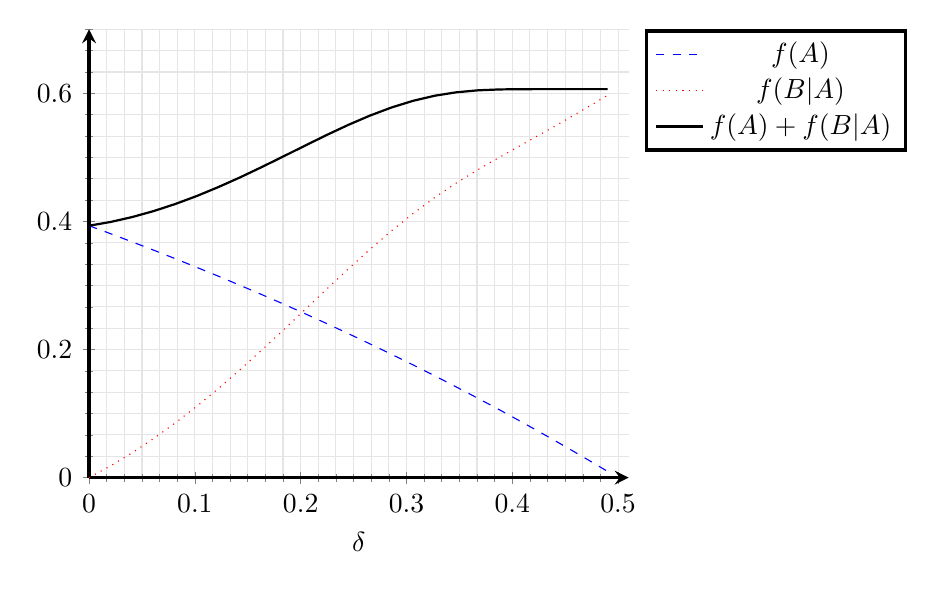
\begin{tikzpicture}
\begin{axis}[
	domain=0:0.49
	,ymax=.7
	,xmax=.51
	,xlabel=$\delta$
	,axis lines=left
	,grid=both
	,grid style={
		draw=gray!20
	}
	,minor tick num=5
	,legend pos=outer north east
	,legend entries={
		$f(A)$
		,$f(B|A)$
		,$f(A) + f(B|A)$
	}
]
  \addplot[blue, dashed, thin]{1-exp(-(0.5-x))};
  \addplot[red, dotted, thin]{(1 - exp(-(4*x/(1-2*x)))) * (exp(-1/2) - 1 + exp(-(1/2-x)))};
  \addplot[black, thick]{1-exp(-(0.5-x)) + (1 - exp(-(4*x/(1-2*x)))) * (exp(-1/2) - 1 + exp(-(1/2-x)))};
\end{axis}
\end{tikzpicture}
\end{figure}



\section{The Modified\textsuperscript{2} Greedy Algorithm}\label{sec:Modified2Greedy}
We now analyze the modified modified greedy algorithm.

Let $\epsilon > 0$ a constant to be determined latter on, and let $T$ be the output of 
the algorithm.

\begin{theorem}
$f(S) \geq 1 - e^{-(1/2 + \epsilon)}$
\end{theorem}

\begin{proof}
We can assume that $f(\{e_1, e_2\}) \leq 1 - e^{-1/2 + \epsilon}$ 
for every $e_1, e_2 \in U$ or otherwise the proof holds.
Note, also, that if $|O \setminus T| \leq 2$ then $f(T) \geq 0.5$.
Thus we assume the algorithm drops at least three elements from $O$ during its running.
Let $x$ be the first element in $O$ that was dropped by the algorithm, 
and let $A$ be the set of elements chosen by the algorithm just before dropping $x$.
If $f(A) \geq 1 - e^{-1/2}$ the theorem holds, 
otherwise denote $f(A) = 1 - e^{-(1/2 + \epsilon - \delta)}$.
We say that an element, $e$, is \emph{expensive} if $c(e) \ge 1/4 + \epsilon/2 - \delta/2$, 
otherwise it is \emph{cheap}.
Observe that $O$ contains at most two expensive elements, thus the algorithm drops 
at least one cheap element from $O$. 
Let $y$ be the first such element, and let $B$ be the set of elements chosen by the 
algorithm right after dropping $x$ and just before dropping $y$.
Also denote by $C$ the subset of cheap elements in $O$, 
i.e. $C = \{e \in O : c(e) < 1/4 + \epsilon/2 - \delta/2\}$.

We argue that the following inequalities hold:

\begin{align}
c(A) \leq 0.5 + \epsilon - \delta 
\\
c(x) > 0.5 -\epsilon + \delta
\\
c(C) \leq 0.5 + \epsilon - \delta
\\
c(B) > 2\delta
\\
f(C) \ge e^{-1/2 + \epsilon}
\\
c(B) \ge 1/4 - 3\epsilon/2 + 3\delta/2
\\
f(B|A) \ge \left[
e^{-(1/2 + \epsilon)}
- (1 - e^{-(1/2 + \epsilon - \delta)})
\right]
(1-e^{-\frac{1-6\epsilon+6\delta}{2+4\epsilon-4\delta}})
\\
f(T) \geq \max_\epsilon \min \{1 - e^{-(0.5 + \epsilon)}, \min_{\delta} f(A) + f(B|A)\}
\end{align}
\todo{explain the inequalities}.

Substituting $f(A) = 1 - e^{-(1/2 - \delta)}$ into the last inequality, 
using $f(B|A) \ge \left[
e^{-(1/2 + \epsilon)}
- (1 - e^{-(1/2 + \epsilon - \delta)})
\right]
(1-e^{-\frac{1-6\epsilon+6\delta}{2+4\epsilon-4\delta}})
$,
and setting (say) $\epsilon = 0.104$ gives the desired result 
as can be seen in Figure~\ref{fig:mmgreedy}.

\end{proof}

\begin{figure}
\def\eps{0.104}
\caption{
\label{fig:mmgreedy}
Modified Modified Greedy Approximation Ratio ($\epsilon = 0.104$)
}
\begin{tikzpicture}
\begin{axis}[
	width=\textwidth
	,domain=0:0.49
	,ymax=.7
	,xmax=.51
	,xlabel=$\delta$
	,xtick distance=0.1
	,ytick distance=0.1
	,axis lines=left
	,grid=both
	,grid style={
		draw=gray!20
	}
	,minor tick num=5
	,legend pos=south west
	,legend entries={
		$f(A)$
		,$f(B|A)$
		,$f(A) + f(B|A)$
	}
]
  \addplot[blue, dashed, thin]{1-exp(-(0.5 + \eps -x))};
  \addplot[red, dotted, thin]{
  	(1 - exp(-(1 - 6 * \eps + 6 * x)/(2 + 4 * \eps - 4 * x)))
  	*
  	(exp(-(0.5 + \eps) - 1 + exp(-(0.5 + \eps - x))))
  };
  \addplot[black, thick]{
  	1-exp(-(0.5 + \eps -x))
  	+
  	(1 - exp(-(1 - 6 * \eps + 6 * x)/(2 + 4 * \eps - 4 * x)))
  	*
  	(exp(-(0.5 + \eps) - 1 + exp(-(0.5 + \eps - x))))
  };
\end{axis}
\end{tikzpicture}
\end{figure}

\paragraph{Upper Bound}
We show that the approximation ratio of the modified modified greedy algorithm is at most $0.5$.
To see this consider the following instance of the budgeted maximum coverage problem:
Let the elements be $X = \{x_1, \dots, x_{2n}\}$, 
and a collection of subsets over $X$, $\mathcal{S} = \{S_1, \dots, S_{n + 1}\} \cup \{S\}$,
where for each $1 \leq i \leq n + 1$, $S_i = \{x_i\}$, and $c(S_i) = 1$. 
Also, set $S = \{x_{n + 2}, \dots, x_{2n}\}$, and $c(S) = n$.
Finally, for each $x \in X$ set $w(x) = 1$ and set the budget for this instance to be $2n$.
One can verify that the modified modified algorithm will return a solution of value $n + 1$
While taking $S$ along with any other $n$ subsets yields a solution of value $2n - 1$.  





\section{Amplification Algorithm}\label{sec:Amplification}
\def\pLarge{P_{\text{large}}}
\def\pVal{P_{\text{val}}}
\def\MGreedy{Modified$^2$Greedy}
\def\BOTAlg{BestOfThree}
\def\mA{\mathcal{A}}

In this section we show a simple algorithm, which given
an $r$-approximation $\mA$ for \SK, $r<1/2$ can
be used to derive an $r'$-approximation, $r<r' <1/2$, for
\SK using  a constant number of calls
for $\mA$ and $\frac{3n^2}{2}+n$ oracle queries.

Algorithm \ref{algorithm:amplify} receives
an approximation algorithm $\mA$ for $\SK$,ƒo
a universe $U$, a monotone non-negative
submodular function $f:2^U \rightarrow \mathbb{R}$,
a non-negative cost function $c:U \rightarrow \mathbb{R}$, and a budget $\beta$.
The algorithm also gets two scalar parameters $\epsilon$
and $\rho$.  These two parameters control the approximation
ratio and complexity of the algorithm, and should be set according
to the claims in this section to obtain the required approximation
ratio and complexity.

Broadly speaking,  the algorithm finds the pair of  elements with maximal value $\pVal$. It then divides all pairs of elements $\{a,b\} \subseteq U$ for which
$\frac{f(\{a,b\})}{f(\pVal)} \geq \rho$ into {\em buckets}, where the subsets
in each bucket have the same value to a factor of $(1+\epsilon)$.
The algorithm then extends the set of smallest cost in  each bucket
to a solution using the algorithm $\mA$.  The algorithm returns the
best between the solutions found using the buckets and $\mA$, the pair of
elements with maximal profit, the single element with maximal profit, and the result of the greedy algorithm
over the input instance.

\begin{algorithm}
	\caption{Amplify($\mA, U, f, c, \beta, \epsilon, \rho$)}
	\label{algorithm:amplify}
	% Initialization
	\tcp{Initialization}
	$\pVal \leftarrow \argmax_{ \{a,b\} \subseteq U, c(\{a,b\})\leq \beta } f(\{a,b\})$
	\\ $w_{\max}\leftarrow f(\pVal)$
	\\ $i_{\max} \leftarrow \floor{\log_{1 + \epsilon} \frac{1}{\rho}}$
	\\
	\tcp{Buckets}
	\For{$i \in \{0,\dots,i_{\max}\}$}{
		$B_i = \left\{ \{a,b\}\subseteq U| c(\{a,b\})\leq \beta, \rho(1+\epsilon)^i \leq \frac{f(\{a,b\})}{w_{\max}}  < \rho (1+\epsilon)^{i+1} \right\}$
		\\
		$P_i \leftarrow \argmin_{\{a,b\}\in B_i} c(\{a,b\})$
%	}
%	\tcp{Candidate Solutions}
%	\For{$i \in \{0,\dots,i_{\max}\}$}{
\\
		$S_i \leftarrow P_i \cup \mA(U , f_{P_i}, c, \beta - c(P_i))$
	}
	$G \leftarrow \text{Greedy}(U, f, c, \beta)$ \label{amplify:greedy}
	\\
	$T \leftarrow \argmax_{\{a\}\subseteq U| c(a)\leq \beta} f(\{a\})$ \label{amplify:singletons}
	\\
	\Return $\argmax_{S \in \{S_0, S_1, \ldots, S_{i_{\max}}, G, \pVal,T\}} f(S)$
	%

\end{algorithm}

The following function, which already appeared on Theorem \ref{thrm:Amplification}, will be useful throughout the analysis of the algorithm:

$$ B(\alpha)=1-e^{-\frac{1}{\alpha}}$$
$$ A(\alpha) = \frac{1}{1-e^{-\alpha}}-\frac{1}{B(\alpha)}$$
 $$D(\alpha)=(1-e^{-\alpha})/B(\alpha)$$

 \begin{lemma}
 	\label{lemma:amplification}
 	Given an $r$-approximation $\mA$ for $\SK$ where $r<\frac{1}{2}$.
 	For any $0< \alpha \leq  \ln 2$, input $U,f,c,\beta$ of $\SK$,
 	and $\epsilon$ such that $0<\epsilon\leq \frac{1-2r}{r}$, then executing
 	Algorithm \ref{algorithm:amplify}  with parameters
 	$(\mA, U, f, c, \beta, \epsilon, A(\alpha))$ returns
 	$$min\left(1-e^{-\alpha}, D(\alpha) + (1-r) \left( \frac{2+\epsilon}{1+\epsilon}(1- D(\alpha)) -1 \right) \right)$$
 	approximation for the input instance.
 \end{lemma}



\begin{proof}

	Fix an optimal solution $O$.
	 If $|O|\leq 2$ the algorithm returns an optimal solution and the Lemma holds.
	Therefore we can assume $|O| \geq 3$.  Denote by $\pLarge$ the set of  two  elements in $O$ with highest cost.
	
	Let $L\beta$ be the highest cost of element in $O$.  If $L\leq 1-\alpha$ then
	by Lemma \ref{lemma:sub-main} and the monotonicity of $f$: $f(G) \geq (1-e^{-\alpha}) f(O)$  (recall that $G$ is the result of
	greedy in line \ref{amplify:greedy} of the algorithm and thus Lemma \ref{lemma:sub-main} can be applied on the appropriate prefix of $G$). Therefore, the algorithm
	returns a solution of value at least $(1-e^{-\alpha})f(O)$ and the Lemma holds. Therefore we can assume  $L> 1-\alpha$.
%
%	{\color{red}
%	consider $G'\subseteq G$ to be the subset selected by the greedy (in line \ref{amplify:greedy})
%	just before the first element from $O$ has been dropped ($G' = G$ if no such element exists).
%	Due to the greedy procedure selection of elements the conditions of Lemma \ref{lemma:sub-main}
%	hold for $G'$ (as $A$)  and $O$ (as $B$), therefore,
%}  $f(G) \geq (1-e^{-\alpha}) f(O)$. Therefore, the algorithm
%	returns a solution of value at least $(1-e^{-\alpha})f(O)$ and the Lemma holds. Hence, we can assume  $L> 1-\alpha$.
	
	If $O\setminus \pLarge \subseteq G$, then
	$f(G)+ f(\pVal)\geq f(O\setminus \pLarge) + f(\pLarge) \geq f(O)$.
	Therefore $f(G)\geq \frac{f(O)}{2}$ or $f(\pVal)\geq \frac{f(O)}{2}$
	thus the Lemma holds (note that $\alpha \leq ln 2$ and therefore
	$1-e^{-\alpha} < \frac{1}{2}$). Thus we can assume that
	$O\setminus \pLarge \nsubseteq G$.
	
	The following corollary states that if $f(\pLarge)$ is fairly small
	with respect to $f(O)$ (equivalently, $f(O|\pLarge)$ is high) then the solution $G$ from the greedy algorithm provides
	the required approximation ratio.
	
	\begin{corollary}
		\label{corollary:cor1}
	If $f(O|\pLarge) \geq D(\alpha) f(O)$ then $f(G)\geq (1-e^{-\alpha})f(O)$.
	\end{corollary}

\begin{proof}
	

	Let $\beta M$ be the third highest cost of element in  $O$.
	As the highest cost of  element in $O$ is $\beta L$,
	using a simple argument we get, $M\leq M(L)$ where $M(L)= \min \{\frac{1-L}{2}, L\}$. Since
	$O\setminus \pLarge \nsubseteq G$, there must be an element from $O \setminus \pLarge$ the greedy in line \ref{amplify:greedy} drops. Since all the elements
	in $O\setminus \pLarge$ are of cost at most $\beta M$ the knapsack must
	already have elements of cost $\beta (1-M)$ at the first time an element from $O\setminus \pLarge$ is dropped. Also, $c(O\setminus \pLarge) \leq \beta(1-L -M)$, therefore by Lemma \ref{lemma:sub-main} and the monotonicity of $f$ we get that:
  	$$f(G)\geq \left(1-e^{- \frac{\beta (1-M) }{c(O\setminus \pLarge)}}\right) f(O\setminus \pLarge)
  			\geq \left(1-e^{- \frac{1-M }{1-L-M}}\right) f(O\setminus \pLarge) .$$
  			
  	We note that the term $\frac{1-M}{1-L-M} = \left(  1- \frac{L}{1-M} \right)^{-1}$ is increasing as a function
  	of $M$  in the range $[0, M(L)]$ (note that $1-L-M >0$ in the range).
  	Therefore $\frac{1-M}{1-L-M} \geq  \frac{1 }{1-L}  \geq \frac{1}{1-(1-\alpha)} = \nicefrac[]{1}{\alpha}$. And conclude
  %	The term  $1-e^{- \frac{1-M(L) }{1-L-M(L)}}$ is increasing as a function of $L$
  %	({\bf this is not trivial, I simply drew the graph on Desmos for that}), therefore
  	%	as $L> (1-\alpha)$ we get
  %		$$f(G)\geq  \left(1-e^{- \frac{1-M(L) }{1-L-M(L)}}\right) f(O\setminus \pLarge)
  	%	\geq \ \left(1-e^{- \frac{1-M(1-\alpha) }{1-(1-\alpha)-M(1-\alpha)}}\right) f(O\setminus \pLarge) $$
  		
  	%As $\frac{2}{3} \leq \alpha \leq \ln 2$ we have $M(1-\alpha) = 1-\alpha$. Combining this with the previous inequality we get
  	  $$f(G)
  	\geq \ \left(1-e^{- \frac{1-M }{1-L-M}}\right) f(O\setminus \pLarge) \geq \left( 1- e ^ {- \frac{1}{ \alpha}} \right)f(O\setminus \pLarge)
  	= B(\alpha)f(O\setminus \pLarge) $$
  	
  	Now, recall that $D(\alpha)= \frac{1-e^{-\alpha}}{B(\alpha)}$,
	$f(O|\pLarge) \geq D(\alpha) f(O)$ by the condition of the
	lemma and $f(O|\pLarge) \leq f(O\setminus \pLarge)$ as
	$f$ is submodular. Using these observations and the last lower
	bound on $f(G)$ we obtain
%	\begin{equation*}
%\begin{array}{rcl}
\begin{align*}
f(G) \geq& B(\alpha)f(O\setminus \pLarge)  \geq
B(\alpha) f(O|\pLarge)\\  \geq&
B(\alpha ) D(\alpha ) f(O)
= B(\alpha)\frac{1-e^{-\alpha}}{B(\alpha) }f(O)= (1-e^{-\alpha})f(O)
\end{align*}
%\end{array}
%	\end{equation*}

	\end{proof}

	\begin{corollary}
		\label{corollary:cor2}
		If $f(G)< (1-e^{-\alpha})f(O)$ and $f(\pVal) < (1-e^{-\alpha})f(O)$ then
		$f(\pLarge) \geq A(\alpha) f(\pVal)$
		\end{corollary}
	\begin{proof}
		As $f(G)< (1-e^{-\alpha})$, the condition of corollary \ref{corollary:cor1} does not hold. Therefore
		$f(O|\pLarge)< D(\alpha) f(O)$. Hence,
		$$f(O)= f(\pLarge) + f(O|\pLarge) < f(\pLarge) + D(\alpha) f(O)$$
		By rearranging the terms and using $f(\pVal) < (1-e^{-\alpha})f(O)$
		we get
		$$f(\pLarge) > (1-D(\alpha)) f(O) > \frac{1-D(\alpha)}{1-e^{-\alpha}} f(\pVal)
		= \left(\frac{1}{1-e^{-\alpha}} - \frac{D(\alpha)}{1-e^{-\alpha}}\right) f(\pVal) = A(\alpha) f(\pVal)$$
		The second inequality uses the observation that $D(\alpha) \leq 1$ for $0\leq \alpha \leq 1$ which can be easily verified. The last equality follows from the definitions
		of $D(\alpha)$ and $A(\alpha)$.
		
			
		\end{proof}

	\begin{corollary}
		\label{corollary:cor3}
			If $f(G)< (1-e^{-\alpha})f(O)$ and $f(\pVal) < (1-e^{-\alpha})f(O)$ then
			there is $i\in \{0, \ldots, i_{\max}\}$ such that
		$$\frac{f(S_i)}{f(O)} \geq D(\alpha) + (1-r)\left( \frac{2+\epsilon}{1+\epsilon} D(\alpha) -1 \right)$$
	\end{corollary}
\begin{proof}
		As the conditions of corollary \ref{corollary:cor2} hold, we have
		$f(\pLarge) \geq A(\alpha) f(\pVal)$.
		 Let $i$ be the minimal integer $i$ such
		that $\frac{f(\pLarge)}{f(\pVal)} < A(\alpha)(1+\epsilon) ^{i+1}$, as $f(\pLarge) \geq A(\alpha) f(\pVal)$ we get $i\geq 0$.
		Recall that $i_{\max}= \floor{\log_{1+\epsilon} \frac{1}{\rho} } =
		\floor{\log_{1+\epsilon} \frac{1}{A(\alpha)}} $ (as the algorithm is used
			with $\rho=A(\alpha)$).
			Therefore,
			$$A(\alpha) (1+\epsilon) ^{i_{\max} +1}
			> A(\alpha) \frac{1}{A(\alpha) } = 1 \geq \frac{f(\pLarge)}{f(\pVal)}$$
			Thus $i\leq i_{\max}$.
			Also $c(\pLarge) \leq c(O) \leq \beta$, and we can conclude that
			$\pLarge \in B_i$ (note that $w_{\max} = f(\pVal)$).
			
			From the definition of $P_i$ we get $c(P_i)\leq c(\pLarge)$ and
			$f(P_i) \geq \frac{1}{1+\epsilon} f(\pLarge)$.
			Let $Q_i  =  \mA(U, f_{P_i}, c, \beta - c(P_i))$.
			As $c(P_i) \leq c(\pLarge)$ we get that $O\setminus \pLarge$
			is a feasible solution for the problem instance given to $\mA$.
			Hence, as $\mA$ is a $r$-approximation we get
			$$f(Q_i | P_i) \geq r f(O\setminus \pLarge| P_i)$$
			Therefore,
			\begin{align*}
			f(S_{i})
			&
			\geq f(P_i) + f(Q_i|P_i)
			\\ &
			\geq f(P_i) + r f(O \setminus \pLarge | P_i)
			\\ &
			\geq f(P_i) + r(f(O) - f(\pLarge) - f(P_i))
			\\ &
			= (1-r)f(P_i) + r(f(O) - f(\pLarge))
			\\ &
			\geq \frac{1-r}{1 + \epsilon}f(\pLarge) + r(f(O) - f(\pLarge))
			\\ &
			= \left(
			\frac{(2 + \epsilon)}{(1 + \epsilon)}(1-r) - 1
			\right)
			f(\pLarge)
			+ rf(O)
			\label{eq:sub:bucket}
			\end{align*}
			
			As $\epsilon\leq \frac{1-2r}{r}$ one can deduce that
			$\left(
			\frac{(2 + \epsilon)}{(1 + \epsilon)}(1-r) - 1
			\right) \geq 0$.
			Also, since $f(G)< (1-e^{-\alpha})f(O)$ by corollary \ref{corollary:cor1} we
			get $f(O|\pLarge)  <D(\alpha)f(O)$, by using $f(O|\pLarge)= f(O) -f(\pLarge)$
			and rearranging  the terms we get
			$f(\pLarge)> (1-D(\alpha)) f(O)$.
			Therefore,
			\begin{align*}
			f(S_i) \geq&
			\left(
			\frac{(2 + \epsilon)}{(1 + \epsilon)}(1-r) - 1
			\right)
			f(\pLarge)
			+ rf(O) \\ \geq &
				\left(
			\frac{(2 + \epsilon)}{(1 + \epsilon)}(1-r) - 1
			\right) (1-D(\alpha ) )f(O) +rf(O)\\
			=& f(O) \left(  D(\alpha) + (1-r)\left(  \frac{(2 + \epsilon)}{(1 + \epsilon)} (1-D(\alpha)) -1\right) \right)
			\end{align*}
			and the corollary immediately follows.
			
		
	\end{proof}
The Lemma follows immediately from corollary \ref{corollary:cor3} as it states
that either $G$, $\pVal$ or $S_i$ for some $i$ would provide the required approximation
ratio.
\end{proof}

\begin{lemma}
	\label{lemma:amp_runtime}
Algorithm \ref{algorithm:amplify} uses $\floor{\log_{1+\epsilon} \frac{1}{\rho}}+1$
	invocation to $\mA$ and up to $\frac{3}{2} n ^2+n$ additional oracle queries.
 \end{lemma}
\begin{proof}
	The number of invocation to $\mA$ immediately follows from the algorithm.
	Beside the invocation to $\mA$ the algorithm runs the greedy procedure
	which uses up to $n^2$ queries. The queries for the initialization and
	buckets phases only considers sets of size $2$, and therefore can be
	implemented by up to $n(n-1)/2\leq n^2/2$ queries. The execution
	of line \ref{amplify:singletons} would take another $n$ queries.
	\end{proof}



\begin{proof}[Proof of Theorem \ref{thrm:Amplification}]
	Let $$\alpha^*  = \argmax _{0<\alpha \leq \ln{2}} \left\{ \min \left\{ 1-e^{-\alpha},D(\alpha)+(1-r)\left( \frac{2+\nu(\alpha)}{1+\nu(\alpha)} (1-D(\alpha)) -1\right)\right\}\right\}$$
	We obtain the described approximation ratio when running the algorithm
	with $\epsilon = \nu(\alpha^*)$ and $\rho = A(\alpha^*)$.
	By the conditions of the theorem,
	$$k \geq -\frac{\log A(\ln 2)} { \log(\nicefrac[]{1}{r} -1 ) } +1 \geq-\frac{\log A(\alpha*)} { \log(\nicefrac[]{1}{r} -1 ) } +1 $$
	Where the last inequality uses the fact that $A$ is monotonically decreasing.  Thus,
	$$\epsilon^* = 2 ^{-\frac{\log_2 (A(\alpha^*))}{k-1}} -1 \leq \
	2 ^{-\frac{ \log_2(A(\alpha^*))}{  -\left(\frac{\log_2(A(\alpha* ))}{\log_2(\nicefrac[]{1}{r}-1)} \right) }} -1  =
	2^{\log_2(\nicefrac[]{1}{r}-1)} -1 = \nicefrac[]{1}{r}-2 = \frac{1-2r}{r} $$
	therefore the conditions of Lemma \ref{lemma:amplification} apply,
	and the approximation ratio follows.
	
	By lemma \ref{lemma:amp_runtime} the number of invocations for $\mA$
	is
	\begin{align*}
	\floor{\log_{1+\epsilon^*} \frac{1}{A(\alpha^*)}}+1 \leq \
	-\log_{1+\epsilon^*} (A(\alpha^*)) +1 =
	\frac{-\log A(\alpha^*)} {\log(1+\epsilon^*)} +1 \\
	= \frac{-\log {A(\alpha^*)}} {\log(2 ^{-\frac{\log_2 (A(\alpha^*))}{k-1}} )} +1
	= \frac{-\log {A(\alpha^*)}} {-\frac{\log_2 (A(\alpha^*))}{k-1}} +1
	= k \end{align*}
	and the number of addition oracle queries is $\nicefrac[]{3n^2}{2} + n $
	as required.
	
\end{proof}

 

\bibliographystyle{plainurl}
\bibliography{main}

\appendix
\section{Omitted Proofs}
\label{appendix:omitted}
\begin{proof}[Proof of Lemma \ref{lemma:sub-main}]
	

		Consider $a_i$ and observe that:
		\begin{align}
		\frac{f(a_i|A_{i-1})}{c(a_i)}c(B)
		& = \sum_{e \in B} \frac{f(a_i|A_{i-1})}{c(a_i)}c(e)
		\nonumber
		\\ 	& \geq \sum_{e \in B} \frac{f(e|A_{i-1})}{c(e)}c(e)
		\label{ineq:main:cond}
		\\	& \geq f(B|A_{i-1})
		\label{ineq:main:sub}
		\\ 	& \geq f(B) - f(A_{i-1}).
		\label{ineq:main:mon}
		\end{align}
		Inequality \eqref{ineq:main:cond} follows from the condition in the lemma, inequality \eqref{ineq:main:sub} follows from the submodularity of $f$, and inequality \eqref{ineq:main:mon} follows from the monotonicity of $f$.
		Thus, from the above we can conclude that:
		$$
		f(B) - f(A_i)  \leq (f(B) - f(A_{i - 1}))
		\left(1 - \frac{c(a_i)}{c(B)}\right).
		$$
		Hence,
		$$
		f(B) - f(A_i)  \leq f(B) \prod_{j = 1}^{i}
		\left(1 - \frac{c(a_j)}{c(B)}\right).
		$$
		Applying the inequality $1 - x \leq e^{-x}$ we get that:
		$$
		f(B) - f(A_i)  \leq f(B)\cdot
		e^{-\frac{c(A_i)}{c(B)}}.
		$$
		Rearranging the terms and setting $i = k$ completes the proof.

	
	
	
\end{proof}





\end{document}
